\chapter{HASIL YANG DIHARAPKAN}

\section{Hasil yang Diharapkan dari Penelitian}

Penelitian ini diharapkan menghasilkan sistem pemantauan komponen \emph{overheat} pada gardu listrik menggunakan robot \emph{quadruped legged} yang dilengkapi dengan kamera termal. Sistem ini diharapkan dapat mendeteksi overheating secara \emph{real-time}, meningkatkan efisiensi dan keamanan pemantauan gardu listrik. Robot diharapkan mampu melakukan patroli mandiri, menghindari rintangan, serta memberikan estimasi posisi dan jenis komponen yang terdeteksi mengalami \emph{overheat}. Selain itu, sistem ini juga diharapkan memungkinkan kontrol jarak jauh melalui antarmuka \emph{web} interaktif, sehingga memudahkan operator untuk mengawasi kondisi gardu listrik tanpa perlu berada di lokasi. Secara keseluruhan, hasil penelitian ini diharapkan dapat meningkatkan keamanan dan efisiensi dalam pemantauan gardu listrik serta memberikan kontribusi pada pengembangan teknologi robotika di sektor kelistrikan.

\section{Hasil Pendahuluan}

Sampai saat ini, peneliti telah melakukan pengujian terhadap berbagai sistem robot. Adapunan hasil yang telah diperoleh adalah sebagai berikut:

\subsection{Pengujian \emph{Localization Node}}
Implementasi program \emph{Localization Node} diuji menggunakan robot \emph{iCar} di kampus ITS. Pengujian dilakukan dengan mengulang rute yang sama sebanyak dua kali untuk memverifikasi presisi estimasi posisi. Hasil pengujian menunjukkan bahwa robot mampu mendeteksi posisinya dengan sangat akurat, terlihat dari kedua pengulangan yang memberikan hasil konsisten dalam hal posisi dan orientasi.

\begin{figure}[H] 
  \centering
  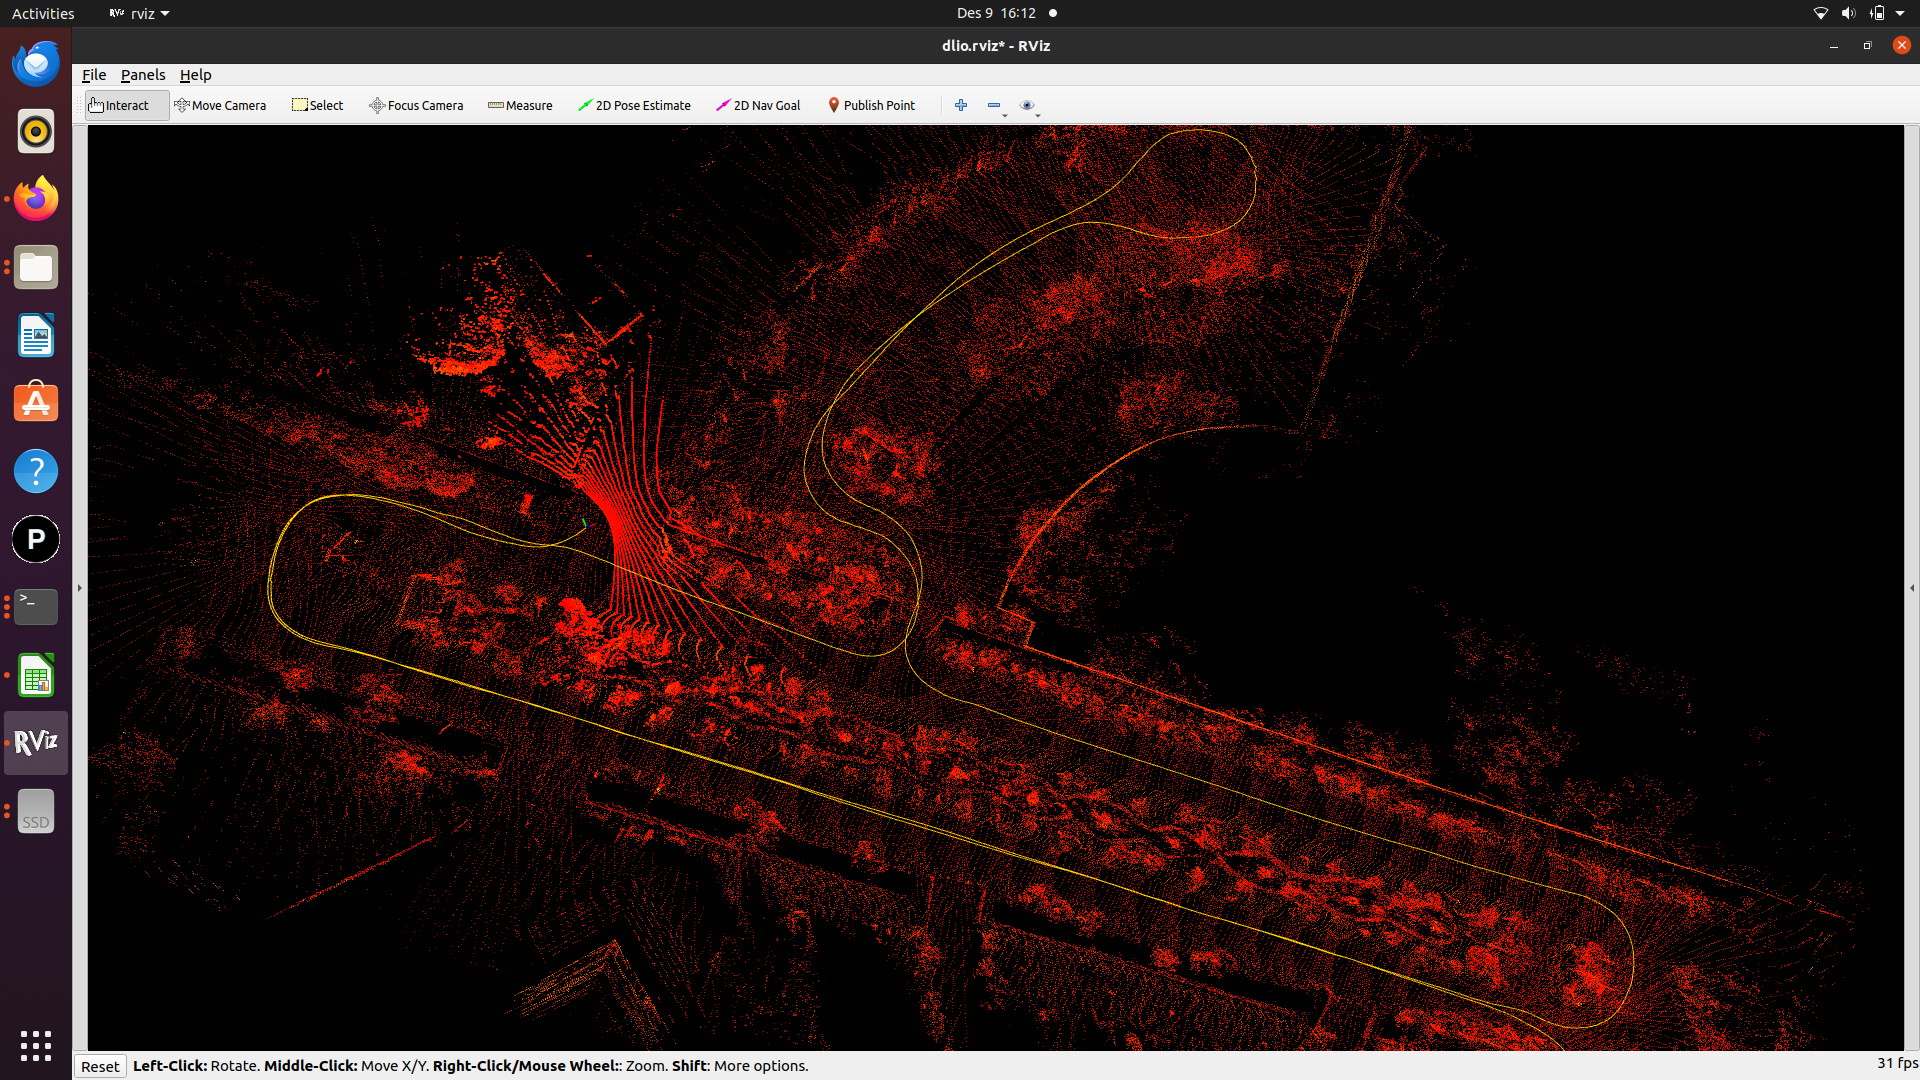
\includegraphics[scale=0.22]{gambar/dlio_its.png}
  \caption{\emph{DLIO} pada jalan kampus ITS}
  \label{fig:DLIO pada jalan kampus ITS}
\end{figure}

Data hasil lokalisasi menggunakan \emph{DLIO} dibandingkan dengan data \emph{GPS RTK} yang terdapat pada \emph{iCar}, menghasilkan grafik seperti pada Gambar \ref{fig:Perbandingan DLIO dan GPS RTK}.

\begin{figure}[H] 
    \centering
    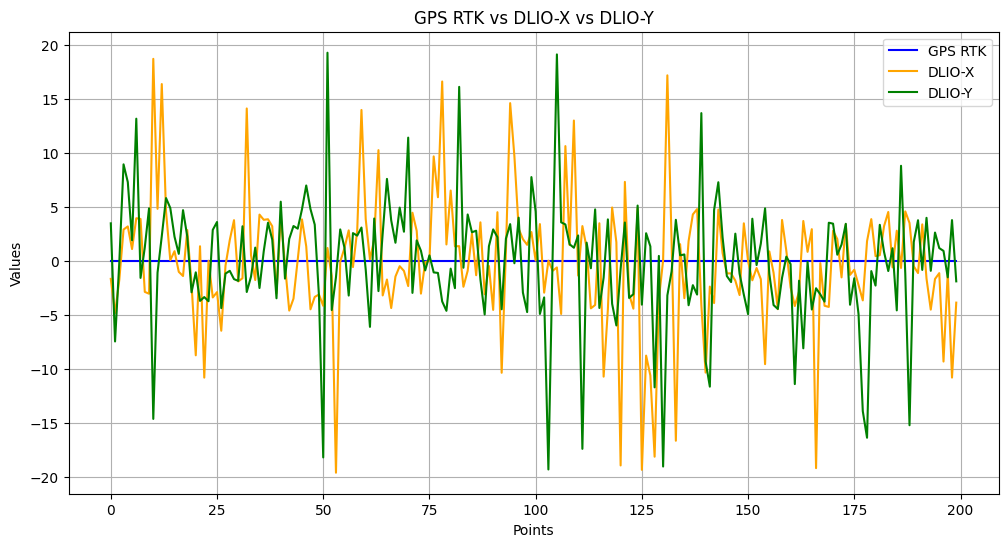
\includegraphics[scale=0.62]{gambar/gpsvsdlio.png}
    \caption{Perbandingan \emph{DLIO} dan GPS RTK}
    \label{fig:Perbandingan DLIO dan GPS RTK}
\end{figure}

Grafik tersebut menunjukkan bahwa hasil lokalisasi \emph{DLIO} memiliki deviasi yang relatif kecil dibandingkan dengan \emph{GPS RTK}, yakni tidak melebihi 20 cm. Meskipun demikian, akurasi dapat ditingkatkan lebih lanjut dengan melakukan \emph{fusion} data IMU dengan \emph{odometry}. Meski begitu, hasil yang diperoleh saat ini sudah cukup memadai untuk digunakan sebagai acuan dalam pengendalian robot.

\subsection{Pengujian Model \emph{Computer Vision}}
Dataset citra termal gardu listrik yang diperoleh dari platform \emph{Roboflow} dilatih menggunakan \emph{YOLOv8} dengan berbagai konfigurasi parameter. Model yang digunakan adalah \emph{YOLOv8s}, dengan jumlah \emph{epoch} 50, 100, 200, dan 300, \emph{batch size} 2, 4, dan 8, serta \emph{optimizer} \emph{Adam} dan \emph{SGD}. Dari kombinasi tersebut, diperoleh 48 model, dan 10 model terbaik berdasarkan nilai \emph{mAP50} disajikan pada Tabel \ref{tab:model_teratas_map50}.

\begin{table}[h!]
    \centering
    \begin{tabular}{|l|c|c|c|c|c|c|}
    \hline
    \textbf{Name} & \textbf{Batch Size} & \textbf{Epochs} & \textbf{\textit{Optimizer}} & \textbf{\textit{mAP50}} & \textbf{\textit{Precision(B)}} & \textbf{\textit{Recall(B)}} \\ \hline
    yolov8s       & 8                   & 100             & SGD                         & 0.810282                & 0.795060                      & 0.711395                   \\ \hline
    yolov8s       & 8                   & 300             & SGD                         & 0.786689                & 0.702299                      & 0.787149                   \\ \hline
    yolov8s       & 4                   & 50              & SGD                         & 0.773952                & 0.772349                      & 0.701915                   \\ \hline
    yolov8s       & 2                   & 50              & SGD                         & 0.773948                & 0.741667                      & 0.737056                   \\ \hline
    yolov8s       & 4                   & 300             & SGD                         & 0.772399                & 0.796335                      & 0.679174                   \\ \hline
    yolov8s       & 2                   & 100             & SGD                         & 0.765646                & 0.859258                      & 0.645118                   \\ \hline
    yolov8s       & 2                   & 300             & SGD                         & 0.764409                & 0.838419                      & 0.654519                   \\ \hline
    yolov8n       & 8                   & 300             & SGD                         & 0.757128                & 0.726358                      & 0.721584                   \\ \hline
    yolov8s       & 8                   & 200             & SGD                         & 0.754204                & 0.826324                      & 0.652525                   \\ \hline
    yolov8s       & 8                   & 300             & Adam                        & 0.752367                & 0.829013                      & 0.670934                   \\ \hline
    \end{tabular}
    \caption{10 Model Teratas Berdasarkan \textit{mAP50}}
    \label{tab:model_teratas_map50}
\end{table}

Hasil ini menunjukkan bahwa model \emph{YOLOv8s} dengan konfigurasi \emph{batch size} 8, \emph{epochs} 100, dan \emph{optimizer} \emph{SGD} memberikan performa terbaik dengan nilai \emph{mAP50} sebesar 0.810282 dan nilai \emph{precision} serta \emph{recall} yang cukup tinggi. Pengujian ini memberikan wawasan penting untuk memilih konfigurasi optimal dalam pelatihan model deteksi objek berbasis citra termal.

Adapun hasil \emph{confusion matric}, \emph{lost function}, serta grafik akurasi dari model tersebut tersebut dapat dilihat pada Gambar \ref{fig:confusion_matrix} dan Gambar \ref{fig:loss_function}.
\begin{figure}[H] 
    \centering
    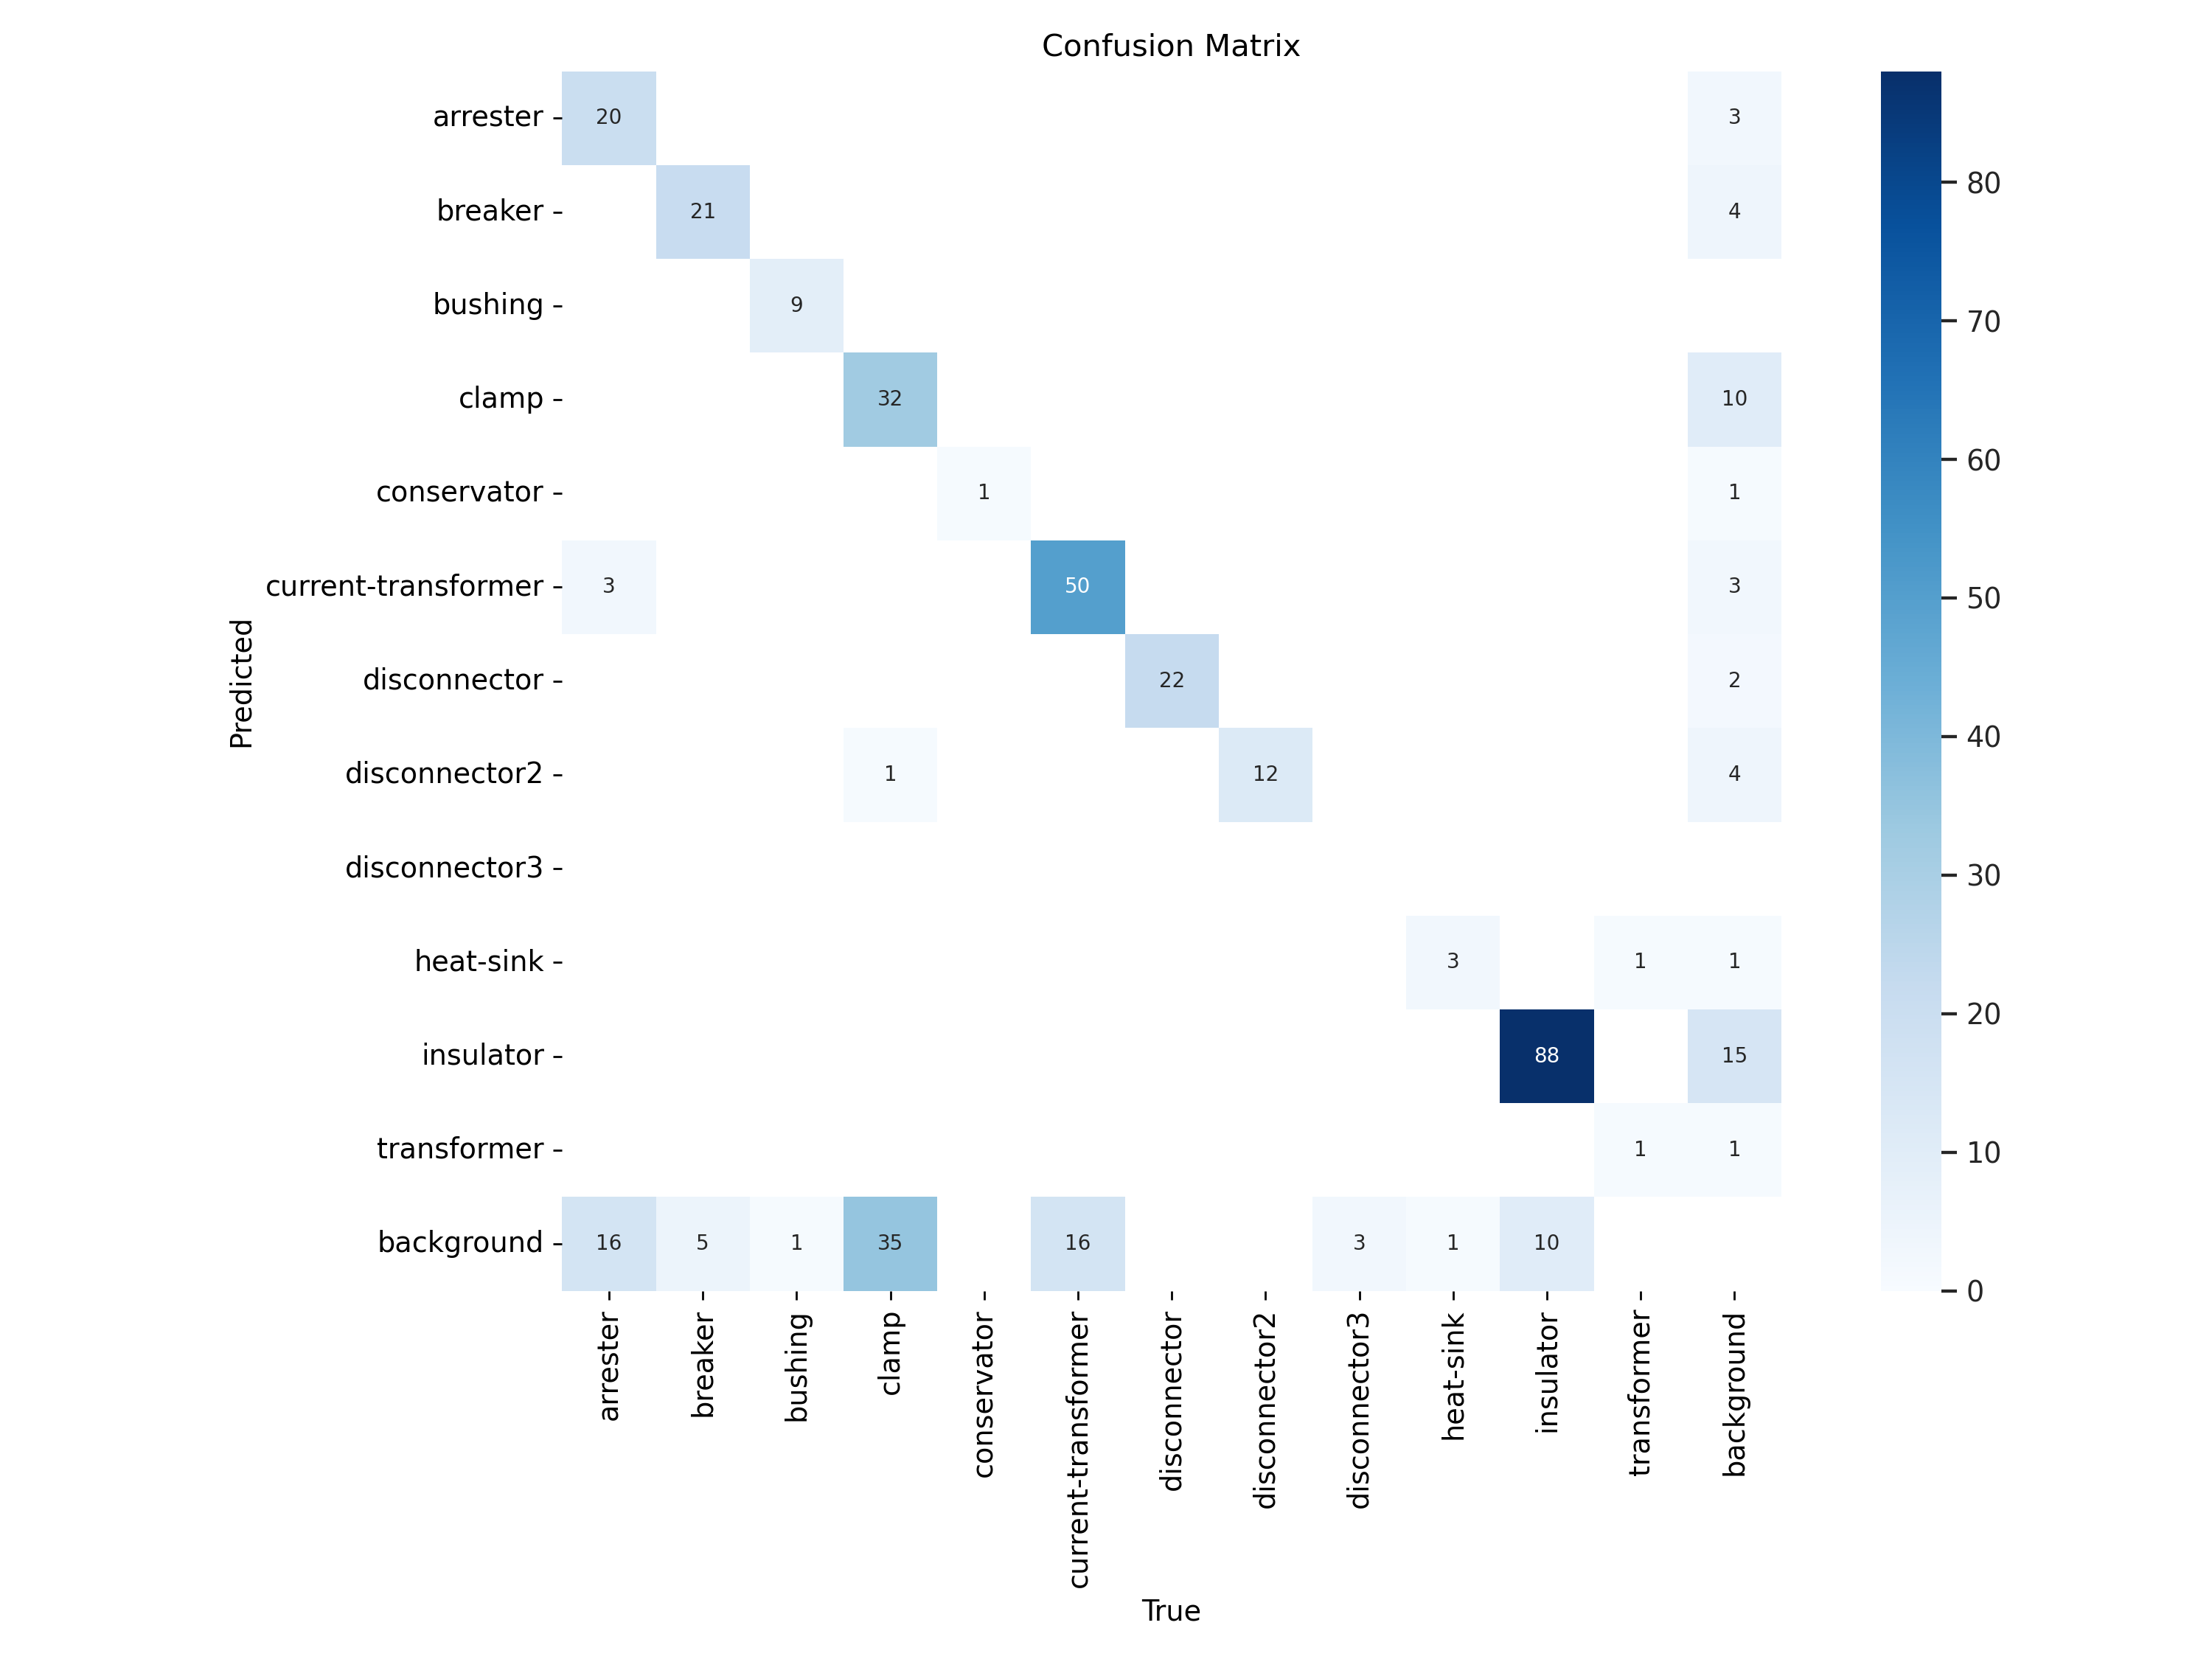
\includegraphics[scale=0.15]{gambar/cf_res.png}
    \caption{\emph{Confusion Matrix YOLOv8n 100 Epoch SGD 8 Batch Size}}
    \label{fig:confusion_matrix}
\end{figure}

\begin{figure}[H] 
    \centering
    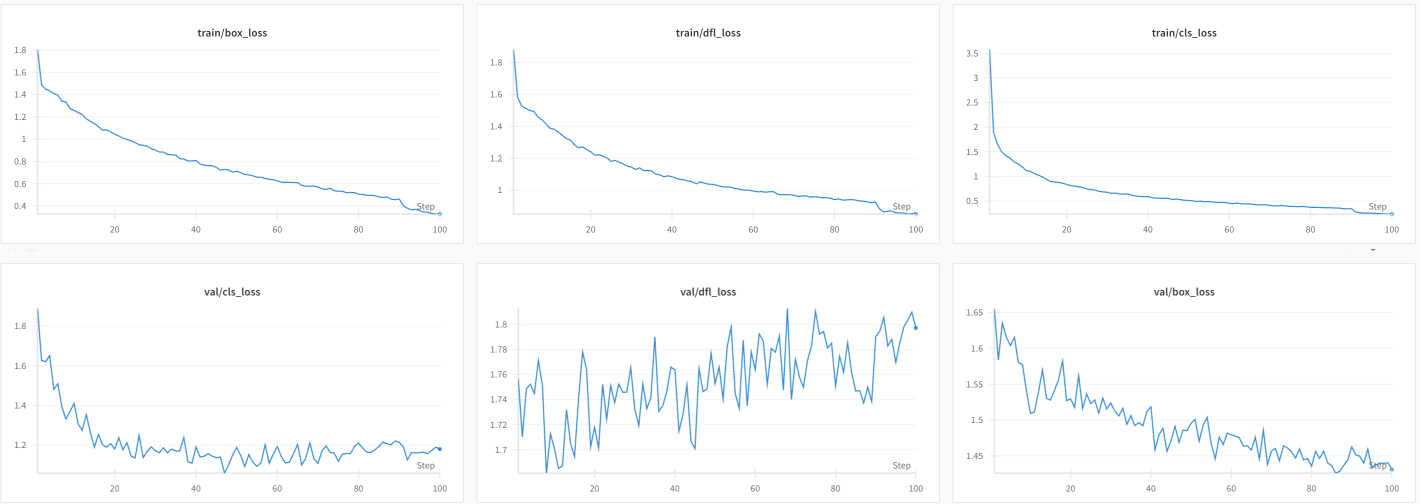
\includegraphics[scale=0.3]{gambar/lost_function.png}
    \caption{\emph{Loss Function YOLOv8n 100 Epoch SGD 8 Batch Size}}
    \label{fig:loss_function}
\end{figure}

Hasil deteksi dari model cukup baik. Ke depannya, performa model akan ditingkatkan dengan pengambilan data langsung dari lingkungan nyata serta penerapan augmentasi pada dataset.

Selain itu, untuk memastikan bahwa model \emph{YOLOv8s} dapat beroperasi pada robot yang menggunakan \emph{mini PC} Jetson Xavier NX 16 GB, dilakukan pengembangan model \emph{YOLO} sederhana dengan konfigurasi parameter pelatihan yang sama, namun dengan kelas yang berbeda. Model tersebut diuji pada \emph{Jetson Nano}, yang merupakan seri di bawah \emph{Jetson Xavier NX}. Hasilnya, model mampu berjalan dengan baik dengan \emph{frame rate per second} (FPS) sebagaimana ditunjukkan pada grafik di bawah.

\begin{figure}[H] 
    \centering
    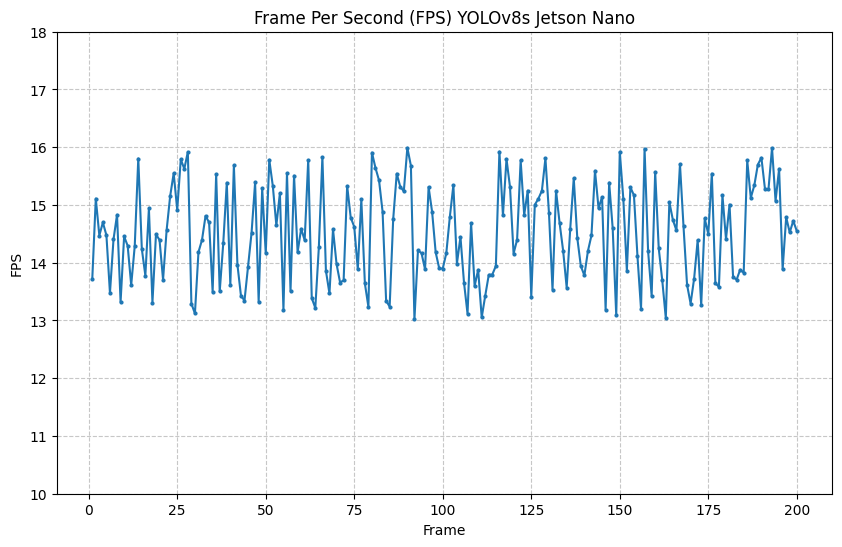
\includegraphics[scale=0.5]{gambar/fps.png}
    \caption{FPS Model \emph{YOLOv8n} pada \emph{Jetson Nano}}
    \label{fig:FPS Model YOLOv8s pada Jetson Nano}
\end{figure}

Dari grafik diatas didapatkan hasil model dapat berjalan di 13 hingga 16 \emph{frame per second} (FPS) pada \emph{Jetson Nano} dengan menggunakan \emph{TensorRT YOLOv8 CPP}. Hasil ini menunjukkan bahwa model akan dapat berjalan dengan baik pada \emph{Jetson Xavier NX} yang akan digunakan pada robot. 

\subsection{Pengujian \emph{Overheat Detection Node}}
Pengujian \emph{overheat detection} dilakukan dengan menggunakan segmentasi HSV pada \emph{bounding box} yang terdeteksi oleh \emph{YOLOv8s}. Pengujian dilakukan pada citra termal gardu listrik yang diperoleh dari platform \emph{Roboflow}. Hasil pengujian menunjukkan bahwa algoritma segmentasi dapat memisahkan area \emph{overheat} dengan baik seperti pada gambar dibawah.
\begin{figure}[H] \centering 
    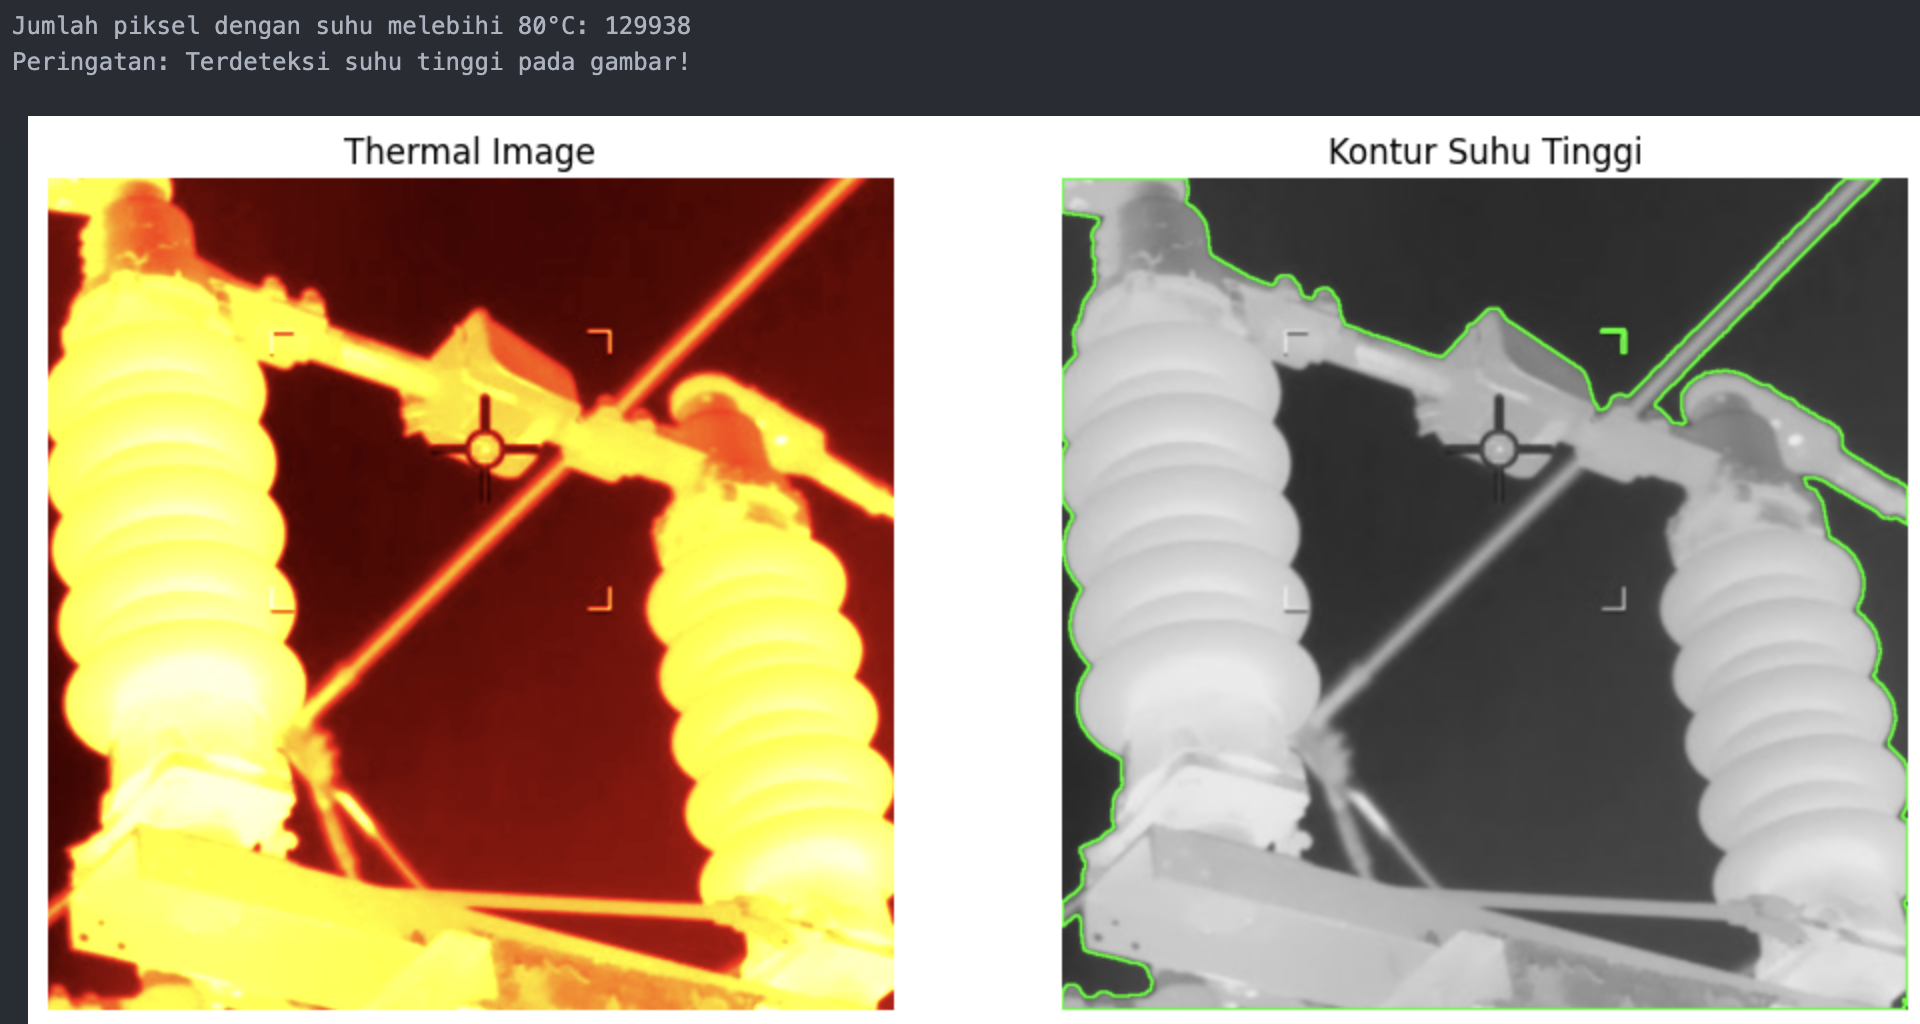
\includegraphics[scale=0.35]{gambar/thermal.png}
    \caption{Pengujian \emph{Overheat Detection} pada citra thermal}
    \label{fig:Overheat Detection pada Robot}
\end{figure}

\subsection{Pengujian \emph{Path Following Node}}

Pengujian \emph{path following} dilakukan untuk menguji kemampuan algoritma dalam menggerakkan robot mengikuti lintasan yang telah ditentukan. Pengujian dilakukan di Taman Alumni ITS dengan rute yang sudah direncanakan sebelumnya. Hasil pengujian menunjukkan bahwa robot dapat mengikuti lintasan dengan baik, meskipun terdapat beberapa deviasi yang dapat diperbaiki dengan penyesuaian konstanta PID. Hasil pengujian dapat dilihat pada Gambar \ref{fig:Path Following pada Robot}.
\begin{figure}[H] \centering 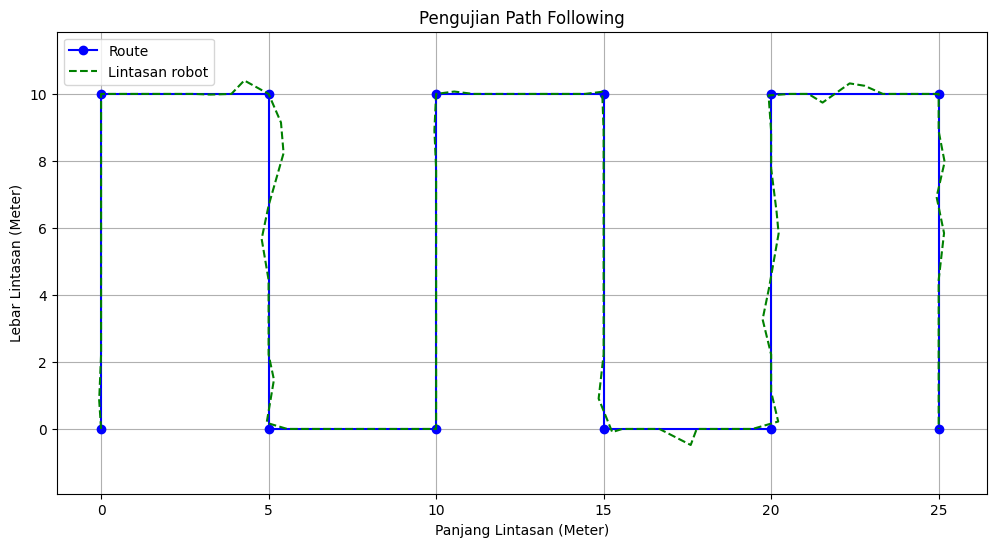
\includegraphics[scale=0.6]{gambar/path_following_test.png} \caption{Pengujian \emph{Path Following} pada Robot} \label{fig:Path Following pada Robot} \end{figure}

Namun, pengujian ini hanya menggunakan data \emph{odometry}, sehingga hasil yang diperoleh belum optimal. Kedepanya data \emph{DLIO} akan digunakan untuk meningkatkan akurasi posisi robot.

\subsection{Pengujian \emph{Obstacle Avoidance Node}}
Pengujian \emph{obstacle avoidance} dilakukan untuk menguji kemampuan algoritma dalam menghindari objek yang ada di lintasan. Pengujian dilakukan dengan mendekatkan sensor pada benda dan sensor dapat memberikan respon untuk menghindar sesuai dengan objek yang terdeteksi sepeti pada gambar 
\begin{figure}[H] \centering 
    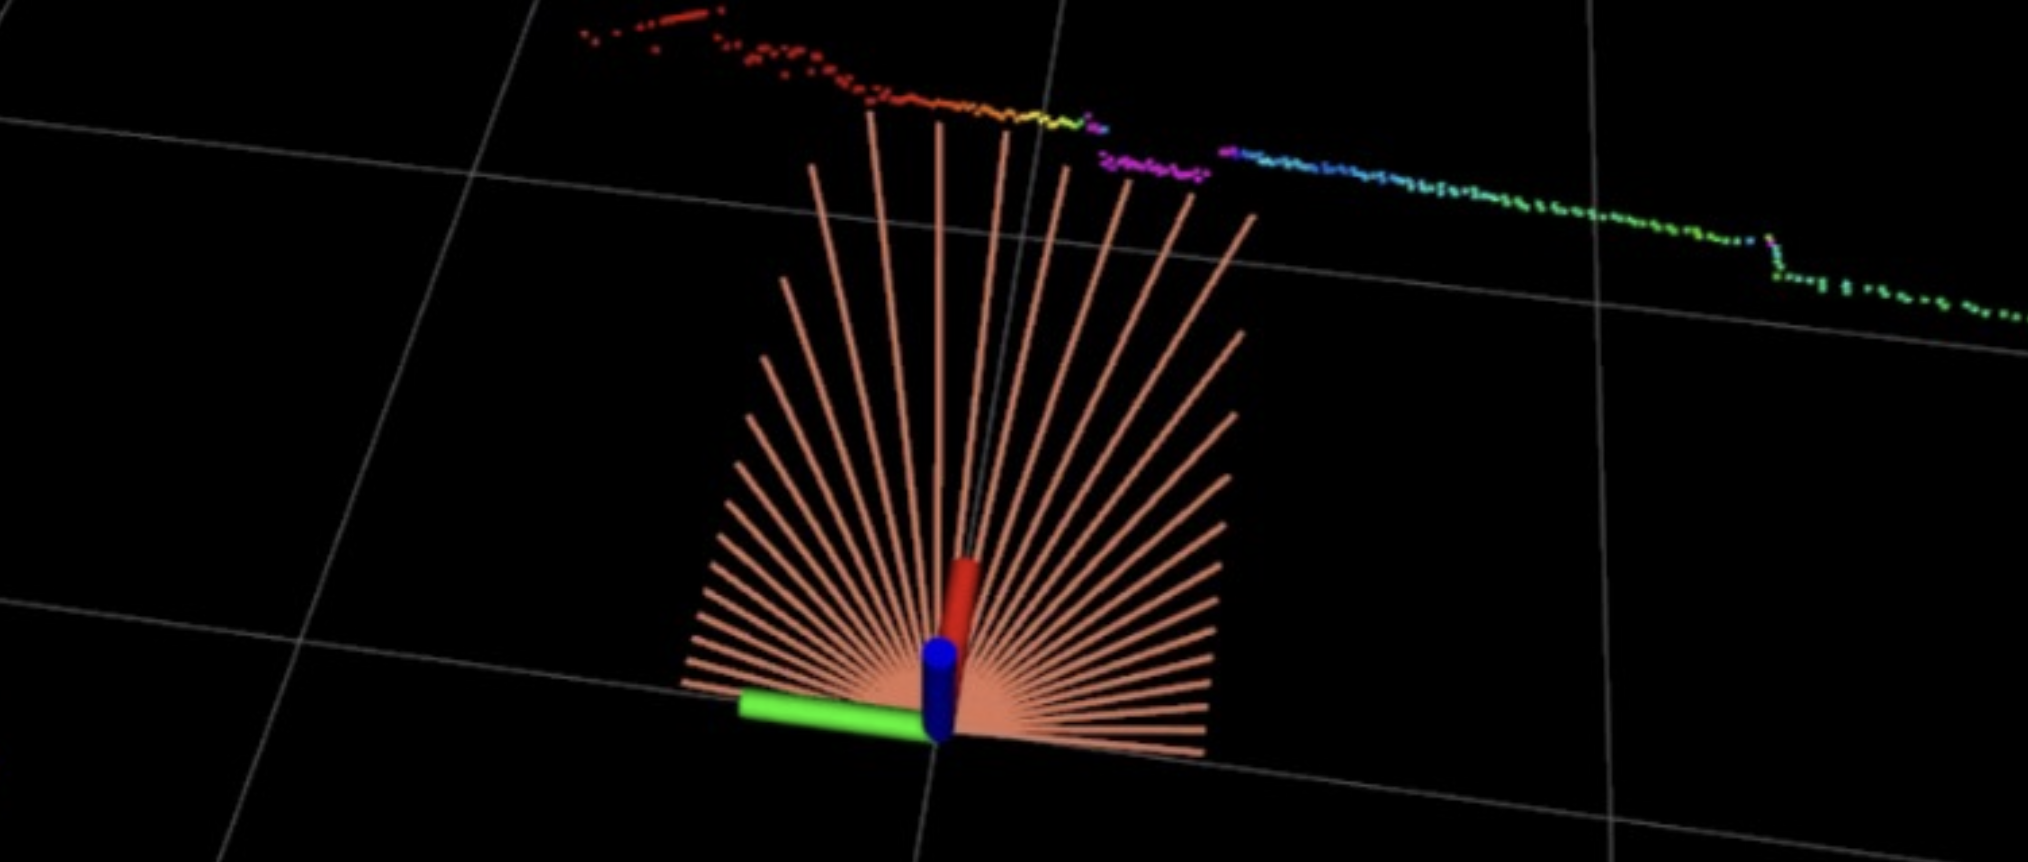
\includegraphics[scale=0.35]{gambar/obstacle_avoidance.png}
    \caption{Pengujian \emph{Obstacle Avoidance} pada Robot}
    \label{fig:Obstacle Avoidance pada Robot}
\end{figure}

